\documentclass[UTF8]{ctexart} % 添加中文支持

% documentclass到begin之间称为导言区,可以在这里进行一些全局设置

% 使用usepackage来添加宏包
% 所谓宏包,就是一系列控制序列的合集,这些控制序列太常用,以至于人们会觉得每次将他们写在导言区太过繁琐,于是将他们打包放在同一个文件中
% 宏包就是用于拓展Latex功能的
\usepackage{graphicx} % 用于导入外部图片的宏包(推荐格式pdf>>>>png>jpg>eps)
\usepackage{amsmath} % 使用 AMS-LaTeX 提供的数学功能
\usepackage{lmodern} % 解决字体警告问题
% \usepackage[pdf]{graphviz} % graphviz绘图支持(需要安装graphviz)
% 我的评价是还不如把latex和graphviz分开使用(latex渲染,graphviz绘图,不必非得把两者合并到一起)
\usepackage{float} % 防止图片乱浮动导致图片文字顺序混乱的包
\usepackage{multirow} % 多行表格合并的宏包
\usepackage{diagbox} % 表头斜线分割宏包
\usepackage{listings} % 代码块宏包
\usepackage{color} % 颜色宏包
\usepackage{arydshln} % 表格虚线宏包
\usepackage{amssymb} % 数学符号宏包

\lstset{
    basicstyle          =   \ttfamily,          % 基本代码风格
    keywordstyle        =   \bfseries,          % 关键字风格
    commentstyle        =   \rmfamily\itshape,  % 注释的风格,斜体
    stringstyle         =   \ttfamily,  % 字符串风格
    flexiblecolumns,                % 别问为什么,加上这个
    numbers             =   left,   % 行号的位置在左边
    showspaces          =   false,  % 是否显示空格,显示了有点乱,所以不现实了
    numberstyle         =   \zihao{-5}\ttfamily,    % 行号的样式,小五号,tt等宽字体
    showstringspaces    =   false,
    captionpos          =   t,      % 这段代码的名字所呈现的位置,t指的是top上面
    frame               =   lrtb,   % 显示边框
}

\title{2021-2022编译原理卷A}
\author{Garone Lombard}
\date{\today}

\begin{document}

% 根据导言区设置生成标题、作者、日期
\maketitle % Insert the title, author and date

\newpage

\begin{abstract}
    编译原理2021-2022试卷答案自行整理
\end{abstract}

\newpage

% 生成目录(需要注意的是,目录的正确生成至少需要编译两次)
\tableofcontents

\newpage

\section{填空}

\paragraph{1.} 编译过程本质上是 \underline{程序转换/翻译}过程,将用 \underline{高级语言}书写的源程序加工为与其等价的目标程序。

\paragraph{2.} 在编译过程的5个基本阶段都要做 \underline{符号表管理} 和 \underline{错误处理} 两件事,因此典型的编译程序常划分为7个逻辑组成部分

\paragraph{3.} 对源程序(包括源程序中间形式)从头到尾扫描一遍,并做有关的加工处理,生成新的源程序中间形式或目标程序,通常称之为 \underline{一遍},完成编译工作最少需要对源程序做 \underline{1} 次扫描

\paragraph{4.} 生产中间代码的目的是便于做 \underline{代码优化} 和 \underline{编译程序移植}

\paragraph{5.} 有文法规则$S\rightarrow if\ E\ S\ |\ if\ E\ S\ else\ S$,用扩充的BNF范式表示为 \underline{$if\ E\ S\ [else\ S]$}

\paragraph{6.} 常见的程序设计语言按乔姆斯基的分类是 \underline{1} 型文法,也称为上下文无关文法。如果采用属性翻译文法处理声明语句$int a;$时,通常可以得到变量类型和名字这样的 \underline{继承} 属性,并填入到 \underline{符号表} 中,以便在使用变量a时,能够查找到变量的有关信息。没有声明就使用变量,这属于 \underline{语义错误} ,在语法分析只能进行句子的结构分析时并不能发现这个问题

\paragraph{7.} 对文法$G[T]:\ T\Rightarrow T-T|T/T|(T)|i$,规范句型$T-T/i$的句柄为 \underline{i} 和 \underline{T-T} ,由此判断该文法 \underline{有} (有/无)二义性。

\paragraph{8.} 规范归约每次归约的是句型的 \underline{句柄} ,算符优先分析法每次归约的是当前句型的 \underline{最左素短语}

\paragraph{9.} 活动记录中Display区存放的是 \underline{各外层模块活动记录的基地址}

\paragraph{10.} 文法$G=(V_n,V_t,P,Z)$,其中$V_t$代表 \underline{文法中的终结符集合}

\section{正则文法与自动机}

\paragraph{题干} 有如下正则表达式

$b*(abb*)*(a|\epsilon)$

\paragraph{1.} 根据正则表达式构造NFA

\begin{figure}[H]
    \centering
    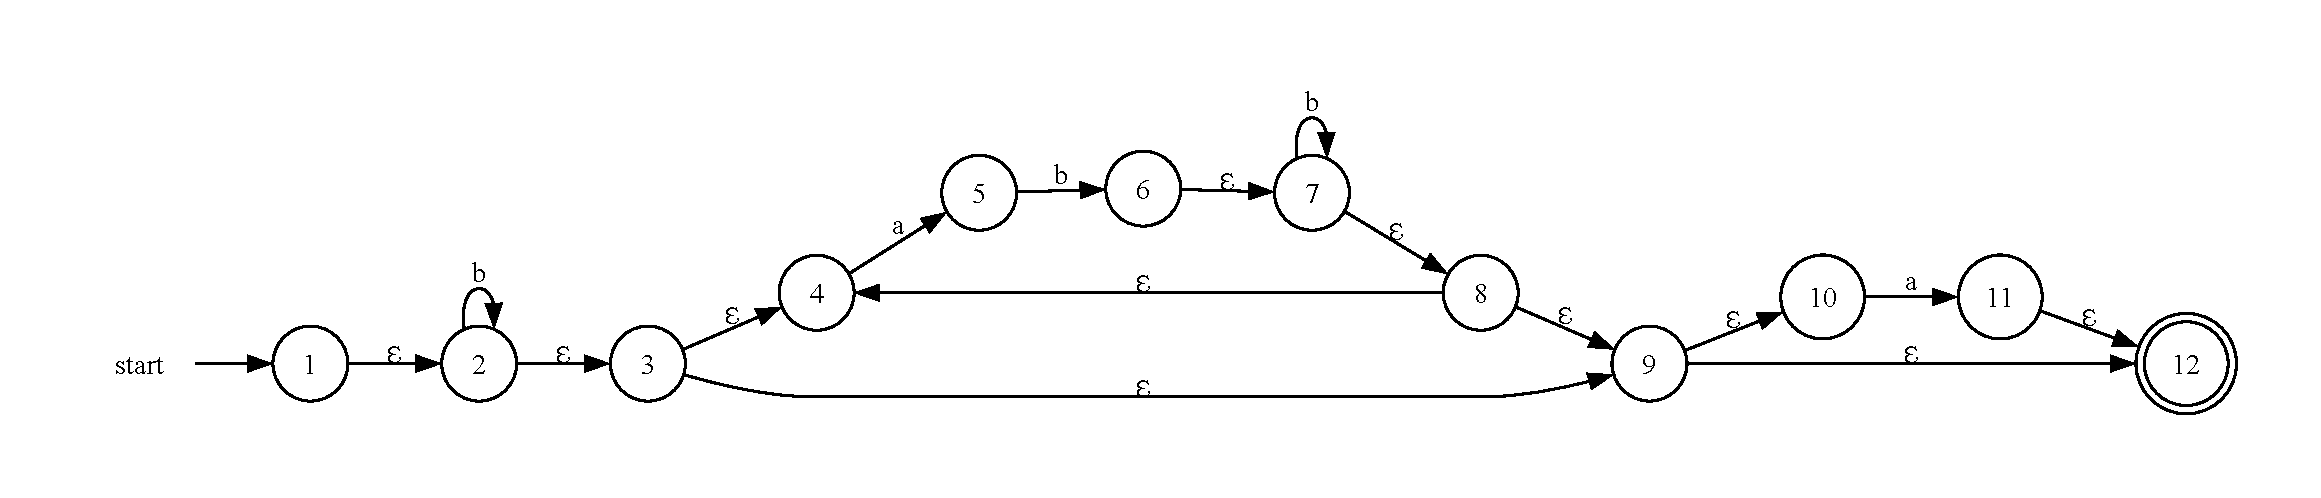
\includegraphics[width=\textwidth]{assets/nfa.pdf}
\end{figure}

\paragraph{2.} 将得到的NFA确定化

\begin{table}[H]
    \centering
    \begin{tabular}{|p{3.4cm}<{\centering}|p{3cm}<{\centering}|p{3.5cm}<{\centering}|}
        \hline
        $\epsilon-closure(start)$ & \multicolumn{2}{c|}{\{1,2,3,4,9,10,12\}}                          \\
        \hline
        \diagbox{状态}{输入}          & a                                        & b                      \\
        \hline
        T0=\{1,2,3,4,9,10,12\}    & T1=\{5,11,12\}                           & T2=\{2,3,4,9,10,12\}   \\
        \hline
        T1=\{5,11,12\}            & $\phi$                                   & T3=\{4,6,7,8,9,10,12\} \\
        \hline
        T2=\{2,3,4,9,10,12\}      & T1=\{5,11,12\}                           & T2=\{2,3,4,9,10,12\}   \\
        \hline
        T3=\{4,6,7,8,9,10,12\}    & T1=\{5,11,12\}                           & T4=\{4,7,8,9,10,12\}   \\
        \hline
        T4=\{4,7,8,9,10,12\}      & T1=\{5,11,12\}                           & T4=\{4,7,8,9,10,12\}   \\
        \hline
    \end{tabular}
    \caption{转换表}
\end{table}

\begin{figure}[H]
    \centering
    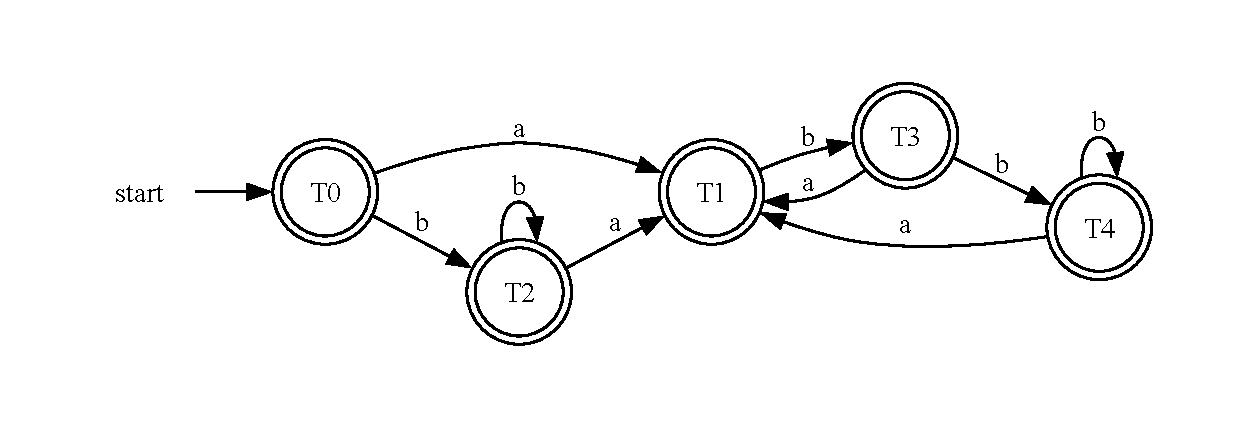
\includegraphics[width=\textwidth]{assets/dfa.pdf}
\end{figure}

\paragraph{3.} 将得到的DFA最小化

\begin{table}[H]
    \centering
    \begin{tabular}{|p{3cm}<{\centering}|p{3cm}<{\centering}|p{3cm}<{\centering}|}
        \hline
        \diagbox{状态}{输入} & a      & b \\
        \hline
        0                & 1      & 2 \\
        \hline
        1                & $\phi$ & 3 \\
        \hline
        2                & 1      & 2 \\
        \hline
        3                & 1      & 4 \\
        \hline
        4                & 1      & 4 \\
        \hline
    \end{tabular}
    \caption{转换表}
\end{table}

显然没有无用状态

首先将状态分为终态和非终态两个集合\{0,1,2,3,4,5\},$\phi$

接下来考察\{0,1,2,3,4,5\}是否可分

\begin{table}[H]
    \centering
    \begin{tabular}{|p{3cm}<{\centering}|p{3cm}<{\centering}|p{3cm}<{\centering}|}
        \hline
        \diagbox{状态}{输入} & a      & b \\
        \hline
        0                & 1      & 2 \\
        \hdashline
        1                & $\phi$ & 3 \\
        \hdashline
        2                & 1      & 2 \\
        \hline
        3                & 1      & 4 \\
        \hline
        4                & 1      & 4 \\
        \hline
    \end{tabular}
    \caption{转换表}
\end{table}

所以可分为\{1\},\{0,2,3,4,5\}两个集合

\begin{figure}[H]
    \centering
    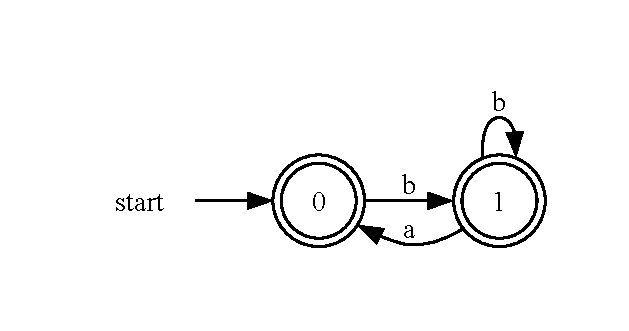
\includegraphics[width=\textwidth]{assets/min-dfa.pdf}
\end{figure}

\section{LL(1)和算符优先分析法}

\paragraph{1.} 证明所有二义性文法都不是LL(1)文法

\paragraph{证明} 二义性文法的句型有两个不同的最左推导,即存在两个不同的最左句型,因此在构造LL(1)分析表时,会出现同一个非终结符对应两个不同的终结符的情况,因此所有二义性文法都不是LL(1)文法

\paragraph{2.} 已知文法G[T]:

\begin{equation}
    \begin{aligned}
        T & \rightarrow T-F|F \\
        F & \rightarrow F/P|P \\
        P & \rightarrow (T)|i
    \end{aligned}
\end{equation}

\paragraph{2.1} 求各文法的FIRSTVT集和LASTVT集

\begin{table}[H]
    \centering
    \begin{tabular}{|p{2cm}<{\centering}|p{1cm}<{\centering}|p{1cm}<{\centering}|p{1cm}<{\centering}|p{1cm}<{\centering}|p{1cm}<{\centering}|}
        \hline
        FIRSTVT & - & / & ( & ) & i \\
        \hline
        T       & 1 & 1 & 1 &   & 1 \\
        F       &   & 1 & 1 &   & 1 \\
        P       &   &   & 1 &   & 1 \\
        \hline
    \end{tabular}
    \caption{FIRSTVT}
\end{table}

\begin{table}[H]
    \centering
    \begin{tabular}{|p{2cm}<{\centering}|p{1cm}<{\centering}|p{1cm}<{\centering}|p{1cm}<{\centering}|p{1cm}<{\centering}|p{1cm}<{\centering}|}
        \hline
        LASTVT & - & / & ( & ) & i \\
        \hline
        T      & 1 & 1 &   & 1 & 1 \\
        F      &   & 1 &   & 1 & 1 \\
        P      &   &   &   & 1 & 1 \\
        \hline
    \end{tabular}
    \caption{LASTVT}
\end{table}

\paragraph{2.2} 构造文法G的优先关系矩阵,并判断该文法是否是算符优先文法

\begin{table}[H]
    \centering
    \begin{tabular}{|p{2cm}<{\centering}|p{1cm}<{\centering}|p{1cm}<{\centering}|p{1cm}<{\centering}|p{1cm}<{\centering}|p{1cm}<{\centering}|}
        \hline
        分析表 & -          & /          & (          & )         & i          \\
        \hline
        -   & $\gtrdot$  & $\lessdot$ & $\lessdot$ & $\gtrdot$ & $\lessdot$ \\
        \hline
        /   & $\gtrdot$  & $\gtrdot$  & $\lessdot$ & $\gtrdot$ & $\lessdot$ \\
        \hline
        (   & $\lessdot$ & $\lessdot$ & $\lessdot$ & $\doteq$  & $\lessdot$ \\
        \hline
        )   & $\gtrdot$  & $\gtrdot$  & err        & $\gtrdot$ & err        \\
        \hline
        i   & $\gtrdot$  & $\gtrdot$  & err        & $\gtrdot$ & err        \\
        \hline
    \end{tabular}
    \caption{分析表}
\end{table}

没有重复的$\lessdot$或$\gtrdot$,因此该文法是算符优先文法

\section{SLR分析法}

\paragraph{题干} 有如下文法G[S]:

\begin{equation}
    \begin{aligned}
        S & \rightarrow CD|DC  \\
        C & \rightarrow aCb|ab \\
        D & \rightarrow Db|b
    \end{aligned}
\end{equation}

\paragraph{1.} 拓展文法,使得文法的开始符号仅出现在一个产生式的左侧;求原文法所有非终结符的FOLLOW集

“使得文法的开始符号仅出现在一个产生式的左侧”:只需构造文法的增广文法即可,如下所示

\begin{equation}
    \begin{aligned}
        S^{'} & \rightarrow S      \\
        S     & \rightarrow CD|DC  \\
        C     & \rightarrow aCb|ab \\
        D     & \rightarrow Db|b
    \end{aligned}
\end{equation}

\begin{table}[H]
    \centering
    \begin{tabular}{|p{2cm}<{\centering}|p{3cm}<{\centering}|p{3cm}<{\centering}|}
        \hline
        集合 & FIRST   & FOLLOW     \\
        \hline
        S  & \{a,b\} & \{\#\}     \\
        \hline
        C  & \{a\}   & \{b,\#\}   \\
        \hline
        D  & \{b\}   & \{a,b,\#\} \\
        \hline
    \end{tabular}
    \caption{LASTVT}
\end{table}

\paragraph{2.} 求拓展后的SLR分析表,包括GOTO表和ACTION表,表头如下

\begin{table}[H]
    \centering
    \begin{tabular}{|p{2cm}<{\centering}|p{1cm}<{\centering}|p{1cm}<{\centering}|p{1cm}<{\centering}|p{1cm}<{\centering}|p{1cm}<{\centering}|p{1cm}<{\centering}|p{1cm}<{\centering}|p{1cm}<{\centering}|}
        \hline
        \multirow{2}{*}{状态} & \multicolumn{3}{c|}{ACTION} & \multicolumn{3}{c|}{GOTO}                   \\
        \cline{2-7}
        ~                   & a                           & b                         & \#  & S & C & D \\
        \hline
        0                   & s1                          & s2                        &     & 3 & 4 & 5 \\
        \hline
        1                   & s1                          & s9                        &     &   & 8 &   \\
        \hline
        2                   & r7                          & r7                        & r7  &   &   &   \\
        \hline
        3                   &                             &                           & acc &   &   &   \\
        \hline
        4                   &                             & s2                        &     &   &   & 6 \\
        \hline
        5                   & s1                          & s10                       &     &   & 7 &   \\
        \hline
        6                   &                             & s10                       & r2  &   &   &   \\
        \hline
        7                   &                             &                           & r3  &   &   &   \\
        \hline
        8                   &                             & s11                       &     &   &   &   \\
        \hline
        9                   &                             & r5                        & r5  &   &   &   \\
        \hline
        10                  & r6                          & r6                        & r6  &   &   &   \\
        \hline
        11                  &                             & r4                        & r4  &   &   &   \\
        \hline
    \end{tabular}
\end{table}

\paragraph{3.} 求能识别规范句型aabbbb活前缀的有效项目集

句柄:ab

活前缀:a,aa,aab

a:
\begin{equation}
    \begin{aligned}
        C & \rightarrow a\cdot Cb \\
        C & \rightarrow a\cdot b  \\
        C & \rightarrow \cdot aCb \\
        C & \rightarrow \cdot ab
    \end{aligned}
\end{equation}

aa:
\begin{equation}
    \begin{aligned}
        C & \rightarrow a\cdot Cb \\
        C & \rightarrow a\cdot b  \\
        C & \rightarrow \cdot aCb \\
        C & \rightarrow \cdot ab
    \end{aligned}
\end{equation}

aab:
\begin{equation}
    \begin{aligned}
        C & \rightarrow ab\cdot
    \end{aligned}
\end{equation}

\newpage

\section{符号表构造与运行时存储分析}

\begin{lstlisting}
program main;
    var x, y : real;
    i, k: integer;
    name: array [1…10] of char;
    procedure P1 (ind:integer);
        var x : integer;
        procedure P2 (j : real);
            procedure P3;
                var f : array [1…5] of integer;
                test1: boolean;
            begin
                ...
            end;{注释:P3}
        begin
            P3;
            ...
        end;{注释:P2}
        procedure P4;
            var r1,r2 : real;
        begin
            r1:=y ;
            r2:=r1+y ;
            P2(r1+r2);
            ...
        end; {注释:P4}
    begin
        P4;
        ...
    end;{注释:P1}
begin
    P1(100);
    ...
end {注释:main}
\end{lstlisting}

\paragraph{1.} 按照以下格式,画出递归下降编译到第21行时,栈式符号表的内容

\begin{table}[H]
    \centering
    \begin{tabular}{|p{1.5cm}<{\centering}|p{1.5cm}<{\centering}|p{1.5cm}<{\centering}|p{1.5cm}<{\centering}|p{1.5cm}<{\centering}|}
        \hline
        序号 & 名字   & 种类   & 类型      & 层号 \\
        \hline
        1  & x    & var  & real    & 1  \\
        \hline
        2  & y    & var  & real    & 1  \\
        \hline
        3  & i    & var  & integer & 1  \\
        \hline
        4  & k    & var  & integer & 1  \\
        \hline
        5  & name & var  & array   & 1  \\
        \hline
        6  & P1   & proc &         & 1  \\
        \hline
        7  & ind  & para & integer & 2  \\
        \hline
        8  & x    & var  & integer & 2  \\
        \hline
        9  & P2   & proc &         & 2  \\
        \hline
        10 & P4   & proc &         & 2  \\
        \hline
        11 & r1   & var  & real    & 3  \\
        \hline
        12 & r2   & var  & real    & 3  \\
        \hline
    \end{tabular}
\end{table}

\paragraph{2.} 运行到第12行时,运行栈的内容如下所示,将空白处填满

\begin{table}[H]
    \centering
    \begin{tabular}{|p{3cm}<{\centering}|p{2cm}<{\centering}|}
        \hline
        test1         &            \\
        \hline
        f             &            \\
        \hline
        f的模板          &            \\
        \hline
        prev abp:abp4 &            \\
        \hline
        ret addr      &            \\
        \hline
        abp4(DISPLAY) &            \\
        \hline
        abp2(DISLPAY) &            \\
        \hline
        adp1(DISPLAY) & abp5: P3   \\
        \hline
        j             &            \\
        \hline
        prev abp:abp3 &            \\
        \hline
        ret addr      &            \\
        \hline
        abp2(DISPLAY) &            \\
        \hline
        abp1(DISPLAY) & abp4: P2   \\
        \hline
        r2            &            \\
        \hline
        r1            &            \\
        \hline
        prev abp:abp2 &            \\
        \hline
        ret addr      &            \\
        \hline
        abp2(DISPLAY) &            \\
        \hline
        abp1(DISPLAY) & abp3: P4   \\
        \hline
        x             &            \\
        \hline
        ind           &            \\
        \hline
        prev abp:abp1 &            \\
        \hline
        ret addr      &            \\
        \hline
        abp1(DISPLAY) & abp2: P1   \\
        \hline
        name          &            \\
        \hline
        name模板        &            \\
        \hline
        k             &            \\
        \hline
        i             &            \\
        \hline
        y             &            \\
        \hline
        x             & abp1: main \\
        \hline
    \end{tabular}
\end{table}

\section{代码优化}

\paragraph{题干} 有如下程序,其中n,m是形参,i,ans,t1,t2,t3,t4,t5,t6,t7,t8,t9都是局部变量

\begin{lstlisting}
    i = 1
    t1 = 0
    ans = 1
L1: if i<=n goto L2
    goto L3
L2: t1 = ans * i
    ans = t1
    t2 = m * t1
    t3 = m / t1
    t4 = t2 + t3
    t5 = t4 * 2
    t6 = m * t1
    t7 = t6 * t6
    t5 = t7 * t6
    t8 = t5
    t9 = t8
    i=i+1
    goto L1
L3: writeln (t8)
    return ans
\end{lstlisting}

\paragraph{1.} 将该代码划分基本块,构造相应的控制流图

\begin{table}[H]
    \centering
    \begin{tabular}{|p{4cm}<{\centering}|}
        \hdashline
        *i = 1               \\
        \hline
        t1 = 0               \\
        \hline
        ans = 1              \\
        \hdashline
        *L1: if i<=n goto L2 \\
        \hdashline
        *goto L3             \\
        \hdashline
        *L2: t1 = ans * i    \\
        \hline
        ans = t1             \\
        \hline
        t2 = m * t1          \\
        \hline
        t3 = m / t1          \\
        \hline
        t4 = t2 + t3         \\
        \hline
        t5 = t4 * 2          \\
        \hline
        t6 = m * t1          \\
        \hline
        t7 = t6 * t6         \\
        \hline
        t5 = t7 * t6         \\
        \hline
        t8 = t5              \\
        \hline
        t9 = t8              \\
        \hline
        i=i+1                \\
        \hline
        goto L1              \\
        \hdashline
        *L3: writeln (t8)    \\
        \hline
        return ans           \\
        \hdashline
    \end{tabular}
\end{table}

\begin{figure}[H]
    \centering
    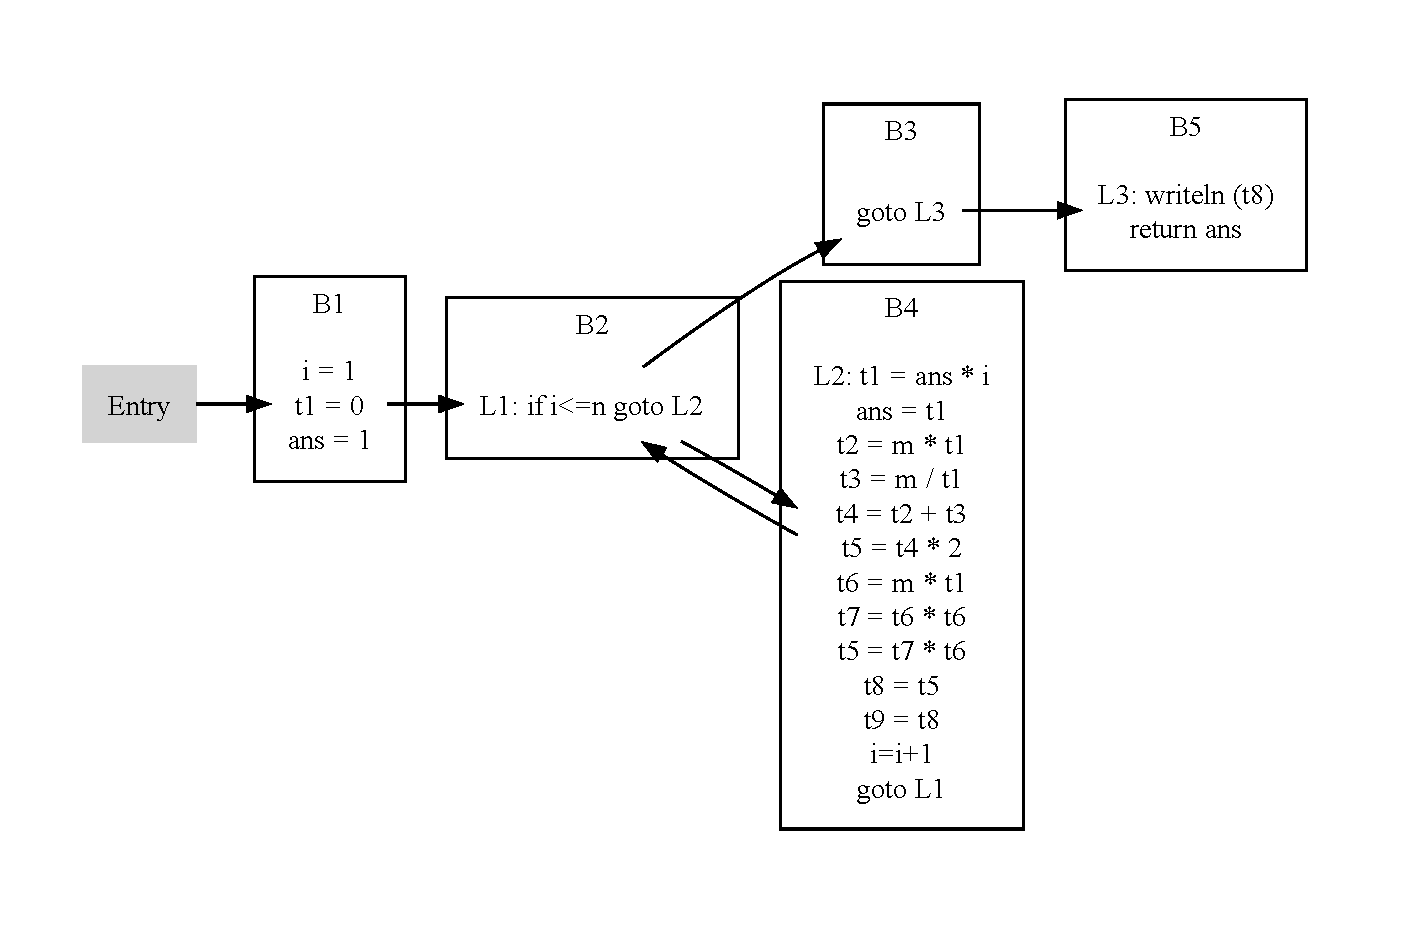
\includegraphics[width=\textwidth]{assets/control-flow.pdf}
\end{figure}

\paragraph{2.} 试对L2所在的基本块用DAG做局部公共子表达式删除优化,并根据启发式算法给出优化后的中间代码序列

\begin{table}[H]
    \centering
    \begin{tabular}{|p{2cm}<{\centering}|p{1cm}<{\centering}|p{1cm}<{\centering}|p{1cm}<{\centering}|p{1cm}<{\centering}|p{1cm}<{\centering}|}
        \hline
        OUT[B] & B1 & B2 & B3 & B4 & B5 \\
        \hline
        i      & 1  &    &    &    &    \\
        \hline
        ans    &    &    &    &    &    \\
        \hline
        n      &    &    &    &    &    \\
        \hline
        m      &    &    &    &    &    \\
        \hline
        t1     &    &    &    &    &    \\
        \hline
        t2     &    &    &    &    &    \\
        \hline
        t3     &    &    &    &    &    \\
        \hline
        t4     &    &    &    &    &    \\
        \hline
        t5     &    &    &    &    &    \\
        \hline
        t6     &    &    &    &    &    \\
        \hline
        t7     &    &    &    &    &    \\
        \hline
        t8     &    &    &    &    &    \\
        \hline
        t9     &    &    &    &    &    \\
        \hline
    \end{tabular}
\end{table}

\paragraph{3.} 给出每个基本块的def和use集合,做活跃变量分析,并给出变量的冲突图。注意:变量A,B冲突的标准为,变量B的定义点处变量A活跃,反之亦然

\end{document}